\chapter{Overview}
\label{ch:overview}

\section{Relational data stores}
\label{sec:relational-data-stores}

\Gls{rdbms} have been the de facto standard for over two decades to efficiently store and query information in a wide variety of native and web applications.
These data stores are based on the relational model devised by Edgar Codd \autocite{Codd1970}.
The data in the system is presented as relations: a collection of data consisting of rows and columns.
The user of the database can query and manipulate the data using relational operators.

Codd presented thirteen rules for a database in order for it to be considered a \textit{relational database} \autocite{Codd1985}.
However, many of the modern database systems do not adhere strictly to all of these rules.
More commonly, a relational database is defined as a database that exposes its information using a collection of rows and columns.

Relational database management systems provide certain guarantees during database transactions.
H\"arder and Reuter discussed recovery in transaction-oriented databases, and introduced the concept of ACID: an acronym referring to a set of transactional properties \autocite{Harder1983}.

\begin{enumerate}
  \item \textbf{Atomicity} \\ Each transaction is ``all or nothing'', either the transaction completes successfully and the data is mutated in an atomic way, or the transaction fails in its entirety and none of the data in the transaction is committed to the database.
  \item \textbf{Consistency} \\ Each transaction, when successful, only commits \textit{legal} results.
        This means that data in the transaction and subsequently in the database does not violate any constraints. The database is always in a consistent state.
  \item \textbf{Isolation} \\ Actions within a single uncommitted transaction are not visible to other, concurrently running transactions.
        Once the transaction has successfully completed, the data is visible for the other transactions.
  \item \textbf{Durability} \\ Once a transaction has completed successfully and been committed to the database, the system must guarantee that these results survive any subsequent malfunction.
\end{enumerate}

\section{NoSQL data stores}
\label{sec:nosql-data-stores}

By 2009, a totally different concept of data storage was popularized \autocite{Leavitt2010}.
NoSQL data stores provide a system of storage that is ``non SQL'' or ``non relational'' \autocite{NoSQL2018}.
Furthermore, properties of NoSQL data stores included horizontal scalability, inherently distributed and open source.
More recently, the NoSQL denomination has also been explained as ``not only SQL'', pointing on the fact that most NoSQL data stores provide a different interface besides SQL.
Many databases expose a REST API as primary execution interface.
Other data stores have devised their own binary communication protocol, such as the Bolt protocol \autocite{Bolt2015} for the Neo4j graph data store.

% MapReduce?
Another concept that became popular together with the increase in dataset size is MapReduce.
MapReduce is a conceptual programming framework and physical implementation for processing big data sets using multiple, distributed nodes \autocite{Dean2008}.
Some NoSQL data stores support this paradigm natively, while others have later added support for it.

The use of non-relational data stores was motivated by the needs of Web 2.0 companies such as Facebook and Google \autocite{Mohan2013}.
NoSQL provides a way to store and process massive amounts of data in a flexible way.
The architecture of such systems is usually more simple than the equivalent relational database systems, and are more aimed at improving horizontal scalability as opposed to vertical scalability.
Data is not stored in rows and columns as is the case in the relational model, but rather in a different data structure.

\textcite{Sadalage2012} reject the proposition that NoSQL data stores replace relational data stores.
Rather, the technology is meant to complement the relational one, and substituting one for another is not deemed to be a potential solution for performance issues.
Since both systems are designed from the ground up with very different ideas in mind, developers have to think about the potential advantages and pitfalls of each.
NoSQL has certain use cases where it shines, whereas the relational data model is a much better fit for other purposes.
The use of multiple data storage technologies and database management systems within the same application is called \textit{polyglot persistence}.

\textcite{Nayak2013} divide the data models used by NoSQL data stores into five categories.
The following sections describe these five categories, and present three additional categories that can be identified in recent NoSQL database trends.

\subsection{Key-value}
\label{subsec:key-value}

Key-value data stores are simple in design, yet powerful and efficient when used in the right circumstances.
A key-value data store allows the user to store schemaless data using an opaque, unique key, creating a \textit{key} and \textit{value} pair.
The values are stored in a manner similar to hash tables or dictionaries commonly found in programming languages and standard libraries.
Queries are processed by looking up the value for the provided key, which is used as an index in the database.
Modern key-value data stores prefer high scalability over consistency, resulting in the fact that more advanced ad-hoc querying and analytical operations on the data such as joins are not supported.

\subsection{Document}
\label{subsec:document}

Document databases store their data in \textit{documents}, indexed by a unique key.
Documents are usually structured in a hierarchical manner and represented in the JSON format.
Document stores are technically a subclass of key-value stores, however the difference lies in the interpretation of the data itself.
In contrast with key-value data stores, the value (document) is not opaque to the database management system, but is parsed and interpreted, and subsequently used for query optimization.
Some document data stores may provide advanced query capabilities on the contents of documents.
Since documents are schemaless, each document may have a similar structure, or a completely different one.

\subsection{Column-oriented}
\label{subsec:column-oriented}

Column-oriented data stores are designed to store data by column rather than by row.
This kind of NoSQL data store is more similar to relational database systems than the other categories, in regard to data structure used to store the data \autocite{Abadi2008}.
In column-oriented data stores, each key is associated with a set of attributes, stored in columns.
Concretely this means that the data is indexed by column value, rather than by row.
Column-oriented data stores are commonly used for queries where only a subset of the attributes is retrieved, as opposed to row-based data stores where the entire row is returned, after possibly discarding any unused values \autocite{Abadi2009}.

\subsection{Graph}
\label{subsec:graph}

Graph data stores keep their data persisted in the form of a graph.
The graph is made up of \textit{nodes} and \textit{edges} as the graph-theoretical model describes \autocite{West2001}.
The former are the database entities that contain the data itself, similar to tables and their respective columns in the relational model.
The latter are the relations between these entities.
Graph data stores use a technique called \textit{index-free adjacency}, where every node contains a logical pointer to the adjacent node \autocite{Weinberger2016}.
This makes graph traversal a very fast operation.
Some graph databases like Neo4j are ACID compliant \autocite{Miller2013}.

\subsection{Object-oriented}
\label{subsec:object-oriented}

Object-oriented data stores represent the data as an object, closely resembling the concept of an object in object-oriented programming languages.
This puts object-oriented data stores much closer to the programming environment than other database systems.
It provides all features inherent to object-oriented languages, such as data encapsulation, inheritance and polymorphism.
The concepts of class, class attributes and an object can be mapped onto the relational concepts of a table, columns and a tuple.
This concept of data storage follows the programming model much better and makes software development more flexible.

\subsection{Multi-model}
\label{subsec:multi-model}

Data stores are generally built and optimized around one data model.
However, databases supporting multiple data models exist as well.
These database systems allow storing data using any of the different data models mentioned before, while integrating these into the same server package.
One example of such a data store is OrientDB \autocite{OrientDB2010}.
Multi-model data stores support and facilitate the principle of polyglot persistence while reducing operational complexity of running multiple database management systems.

\subsection{NewSQL}
\label{subsec:newsql}

NewSQL is a type of relational database management system that aims to provide the same scalability and distributed performance of NoSQL data stores \autocite{Grolinger2013}.
NewSQL data stores are ACID compliant.

\subsection{Triple store}
\label{subsec:triple-store}

A triple store is a type of data store similar to key-value and graph data stores.
Triple stores process data using semantic queries on data triples.
A triple consists of a \textit{subject}, an \textit{predicate} and an \textit{object} \autocite{Rohloff2007}.

\clearpage{}

Most NoSQL data stores are built around the concept of \textit{eventual consistency} \autocite{Brewer2000}.
This is a consistency model that dictates that all accesses to a particular piece of data will eventually return the last updated value.
This principle is broadly implemented in distributed computing systems.
Systems providing this property are also classified as BASE: Basically Available, Soft state, Eventual consistency.
In contrast to the ACID properties, systems built around the BASE principles prefer availability over consistency.

In 2000, Eric Brewer presented a conjecture known as the CAP theorem \autocite{Brewer2000}.
This conjecture, later formally proven \autocite{GilbertLynch2002}, asserts that it is impossible for a distributed data store to exhibit more than two out of three of the following properties:

\begin{enumerate}
  \item \textbf{Consistency}: Every read operation receives the most recent write result
  \item \textbf{Availability}: Every request receives a non-error result
  \item \textbf{Partition tolerance}: The system continues to work despite failure to communicate between nodes
\end{enumerate}

\begin{figure}[H]
  \centering
  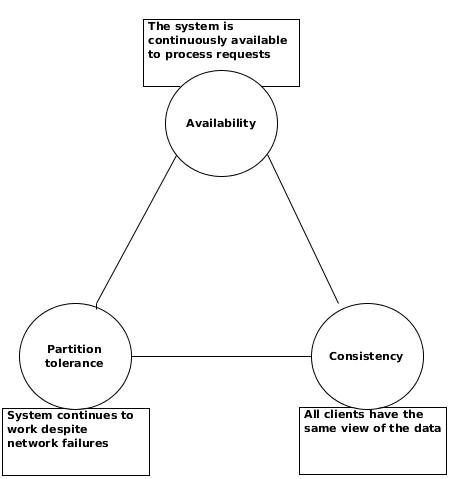
\includegraphics[width=.6\textwidth]{img/cap-theorem.png}
  \caption{CAP Theorem}
  \label{fig:cap-theorem}
\end{figure}

The CAP theorem states that when a network partition is present, the database developer has to choose between providing consistency or availability.
Note that \textit{consistency} as defined by the CAP theorem is not the same concept as consistency as described by the ACID properties.
Database systems respecting the ACID guarantees choose consistency over availability, while database systems built on the BASE principle generally choose availability over consistency.
